\documentclass[10pt,a4paper,twocolumn]{article}

\usepackage{unicode-math}
\setmainfont{Libertinus Serif}
\setmathfont{Libertinus Math}

\usepackage{polyglossia}
\setdefaultlanguage{english}

\usepackage{booktabs,makecell}
\usepackage[binary-units=true]{siunitx}
\usepackage[autopunct=true]{csquotes}
\usepackage[labelfont=bf]{caption}
\usepackage{enumitem}
\setlist{itemsep=0.3ex}
\setlist[enumerate]{label = (\alph*)}
\usepackage[backend=biber,style=alphabetic]{biblatex}
\usepackage{mathtools}
\usepackage{stfloats}
\usepackage{tikz,pgfplots}
\pgfplotscreateplotcyclelist{mylist}{%
    draw={rgb,1:red,0.368417;green,0.506779;blue,0.709798},thick\\%
    draw={rgb,1:red,0.880722;green,0.611041;blue,0.142051},thick\\%
    draw={rgb,1:red,0.560181;green,0.691569;blue,0.194885},thick\\%
    draw={rgb,1:red,0.922526;green,0.385626;blue,0.209179},thick\\%
    draw={rgb,1:red,0.528488;green,0.470624;blue,0.701351},thick\\%
}

\output\expandafter{\the\output\floatfix}

\makeatletter
\def\floatfix{%
\expandafter\ifx\csname r@x@one\endcsname\relax
\else
\ifnum\c@page=\numexpr\expandafter\expandafter\expandafter
              \@secondoftwo\csname r@x@one\endcsname-1\relax
\aftergroup\figone
\fi
\fi}
\makeatother

\renewcommand{\mktextquote}[6]{#1#2#4#5#3#6}


\title{Evaluation of proof-of-ownership countermeasure against off-topic data inclusion attacks in Bitcoin}
\author{Anton Ehrmanntraut}

\renewenvironment{abstract}
{\begin{quote}
\noindent {\bfseries \abstractname.}}
{\end{quote}
}

\begin{document}

\raggedbottom
\maketitle
\begin{abstract}
\end{abstract}

\section{Introduction}

\section{Motivation and Scope}

\begin{table*}
    \centering
    \begin{tabular}{lll}
        \toprule
        \textbf{Address} & \textbf{private key} & \textbf{public key} $f(x)$ \\
        \midrule
        P2PK & $x\in [0{:}2^{256}]$ & $x\cdot G$ \\
        P2PKH & $x\in [0{:}2^{256}]$ & $H(x\cdot G)$ \\
        P2SH* & $x\in [0{:}2^{160}]$ & $H(x)$ \\
        \bottomrule
    \end{tabular}
    \caption{Overview of the discussed address types.}
\end{table*}

% ignore input-script-insertions <-> assume non-standard scripts banned
% P2SH-method uses non-standard script and is not suited for analysis(?)
% required unlocking input however provably is a  public key

% P2MS??

\section{Background}

%Many extensions are discussed that attempt to mitigate the problem of off-topic data inclusion, which, as was outlined in the introduction, can cause unwanted vulnerabilities to the Bitcoin blockchain.
%We focus on proof-of-ownership countermeasures, since that method appears to be the strongest while respecting the principles of the Bitcoin network (permissionless, irreversible, etc.) 
The following section first gives a detailed definition of the proof-of-ownershop countermeasure. After specifying the functionalty and demonstrating its intended effect, we develop an efficient brute-force method to circumvent this countermeasure. Last part of the section gives details on how to implement such circumvention in practice.

\subsection{Proof-of-ownership countermeasure}

In his Master's thesis \emph{Hardening Bitcoin against off-topic data inclusion}, Seeg proposes a countermeasure to this problem using a proof-of-ownership mechanism, which he calls \textquote{preimage solution}. 
He observes that \textquote{variants that store data in standard transactions output can be mitigated by requiring proof that the variable parts}, that is, public keys (P2PK), public key hashes (P2PKH), script hashes (P2SH), \textquote{of the standard transactions are clean.}

He considers an address as clean (i.e.\@ without arbitrary data) if and only if the owner of that address can prove control, that is, ownership of the address.
Such proof of ownership is derived from the \textquote*{private} preimage part of the address, similar to a classic challenge–response authentication.
The wanted effect follows from the assumption that given \textquote*{public} part of a non-clean address, one cannot efficiently derive \textquote*{private} preimage required for the proof of ownership.

For P2PK address types, this translates into a proof using signatures, which certify the control of the corresponding private key.
That is, in order for Alice to send coins to Bob, he sends her off-band his public key $x\cdot G$, and a signature $\sigma$ verifying message $m=H(x\cdot G)$, generated using private key $x$.
Then, Alice can construct a P2PK transaction with recipient key/address $x\cdot G$, and when submitting the transaction to the network, she attaches $\sigma$ which proves that Bob indeed controls that address. 
Miners can verify $\sigma$ using the public key $x\cdot G$ embedded in the transaction, approving the output address of the transaction.

This countermeasure protects against data inclusion: if an adversary wishes to embed message into public key $x\cdot G$, he cannot efficiently derive $x$, required in order to sign the proof $\sigma$.
Thus, given valid $\sigma$, the transaction in question can be safely included into the blockchain.

In the case of P2PKH and P2SH addresses, proofs are constructed in a similar manner.
For P2PKH addresses $H(x\cdot G)$, signed message $m$ remains identical.
Only the public key $x\cdot G$ is additionally transfered such that $\sigma$ can be verified by the network.
For P2SH addresses $H(s)$, the redeem script $s$ serves as preimage/proof $\sigma$.
Again, this prevents data inclusion due to the one-way property of hash function $H$.
(Note that in the case of P2PKH and P2SH transactions, Seeg proposed a slightly weaker approach, exploiting the choice of $H$ as composition of two hash methods, and using the first digest as $\sigma$.)

In fact, this type of countermeasure appears to be one one of the strongest, while (a) not relying on heuristics detecting data inclusion attempts \emph{before} submission into the blockchain, (b) requiring no modifications \emph{after} submission to the blockchain, and (c) retaining the permissionless, pseudonymous nature of the network.
Addresses that withstand the proposed test seem to be precicely the addresses that can be generated by honest participants of the network, who should not be penaltized by any countermeasure.
This further motivates an evaluation of the proposed countermeasure.
Additionally, other countermeasures that respect these mentioned principles build on top of the one-way property of the same cryptographic functions in a similar matter, e.g.\@ \textquote{self-verifying account identifiers} proposed by Matzutt et al.
Therefore, this countermeasure and the respective circumvention act as representative for all one-way-based approaches.

% \subsection{Commitment-based countermeasure}
% TODO Matzutt??

\subsection{Circumvention using partial preimages}

% Refer to similarities between Seegs proofs and Matzutts ICs

In essence, the proposed countermasure builds upon preimage resistance of specific cryptographic one-way functions,
in order to embed identifiers into transactions, that are provably clean by proving existence of the preimage.
That is, for given function $f$, preimage $x$ cannot be efficiently derived from image $f(x)$, whereas only $f(x)$ is stored in the blockchain.
Attempts to embed $y=f(x)$ hence become computationally hard.
The countermeasures use the (presumed) one-way property of Bitcoin's hash function and elliptic curve multiplication.
Incidentally, they correspond to the exact function translating a private key $x$ into a public key resp.\@ address $f(x)$.
Refer to table \ref{} \dots % TODO

No matter the chosen function $f$, the trivial approach to find a preimage to value $y=f(x)$ is via \emph{brute force}: we test pairwise different preimage candidates $x_1, x_2, \dots$ until we find $x_i$ such that $f(x_i)=y$.
The preimage $x_i$ can then be used to generate suitable proofs for the image (e.g.\@ signatures $\sigma$).
Nevertheless, successfully executing such a preimage attack is highly unlikely – in fact, if that attack were possible, an adversary could gain control of the funds assigned to any public key (by inverting the public-key function $f$).

While a full preimage attack is out of reach, \emph{partial} preimage attacks are achievable nontheless:
Given a prefix bitlength $n$, we define $x$ as \emph{partial preimage} of $y$ when $f(x)$ equals $y$ \emph{in the first $n$ leftmost (most significant) bits}, i.e.\@ $f(x)=y\|z$ where $z$ is an arbitrary suffix.

For uniformly chosen private key $x$, we can assume that the respective $n$-bit prefix of the public key $f(x)$ is again uniformly chosen from the range $[0{:}2^n]$.
By this, the success probability of a successful partial preimage attacks increases to $1/2^n$, which, after sufficiently many repetitions and sufficiently small $n$, leads to suitable partial preimage $x$; the corresponding public key $f(x)$ then contains the wanted payload $y$ as prefix.
In terms of the proposed countermeasure, one would continue by constructing transaction containing output address $f(x)$ and proof $\sigma$ from $x$.
Submitting both would then successfully circumvent the countermeasure and include $y$ into the blockchain.

While the notion of prefixes is clear in the case of hash digests involved in P2PKH and P2SH addresses, such prefix of a public key $x\cdot G = (a,b) \in \mathbb{F}_p^2$ involved in P2PK addresses is not neccessarily obvious.
To be definite, we define the $n$-bit prefix of $x\cdot G$ as the $n$ most significant bits of first coordinate $a$ of that curve point. 
(From the perspective of the SEC-defined curve point representation used in Bitcoin, this corresponds to bits 9 to 264. In fact, first byte of the SEC representation is fixed.)


\subsection{Implementation}

Having provided a framework showing the mathematical possibility to circumvent such countermeasure, following section describes the neccessary steps to perform such inclusion in practice.
That is, including payload data in order into the blockchain, where the data is embedded into output addresses of transactions.
Additionally, following procedure generates private keys to each of the used output addresses, such that proofs of ownership can be deduced as required in the countermeasure, and hence the generated transactions are approved.
It is to be noted, that, in the context of Seeg's proposal, investing in a rainbow table could significantly increase performance in comparison to a full brute force approach.
Nevertheless we omit rainbow tables, since this issue could easily be solved when refining the countermeasure, e.g.\@ including transaction hash in the proof message $m$ to be signed.
Cf.\@ with the \textquote{freshness property} in Matzutt's approach.

The procedure is given with a chosen prefix length $n$. Performance and cost directly depend on this parameter, and a fit choice for $n$ is discussed in the next section.

\emph{Preparation.} First, we partition the payload into fragments $y_1, y_2, \dots, y_p$ of length $n$, and use a binary tree as efficient data structure to access the fragments, sorting them by their lexicographic order.

\emph{Partial preimage loop.} 
Then, we have to find a suitable partial preimage $x_i$ for every fragment $y_i$ with $1\leq i \leq p$ in the tree.
In each iteration (of the outer loop), we generate many private key candidates $x$ by brute force (inner loop), until the prefix of $f(x)$ matches any fragment remaining in the tree.
We then can assign matching fragment $y_i$ the private key $x_i \coloneqq x$.
This leads to a mapping $y_i \mapsto x_i$ for all $1\leq i\leq p$.

The implementation is trivial for the P2SH method: let $s$ be an injective function transfering a nonce $m$ into a valid redeem script.
We start off with a random nonce $m$, and test $H(s(m))$, increment $m$, test again, and so forth.
Having found $m$ with prefix of $H(s(m))$ matching one fragment in the tree, we can assign that fragment the private key $s(m)$.

In the case of the P2PK method, this translatest to testing products $m\cdot G$, $(m{+}1)\cdot G$, $(m{+}2)\cdot G,\dots$ from random starting nonce $m$.
Using the axioms of the group formed by the elliptic curve, we can avoid costly elliptic curve multiplications: starting with random nonce $m$, we cache public key $P\coloneqq m\cdot G$.
When incrementing $m$, we add generator point to $P$, that is $P\coloneqq P+G$, and ensure invariant $P= m\cdot G$.
Again, having found $m$ with prefix of $P$ matching one fragment in the tree, we assign that fragment private key $m$.
The P2PKH method can be implemented similiarly, by testing hashes $H(P)$.

\begin{figure*}
    \centering
    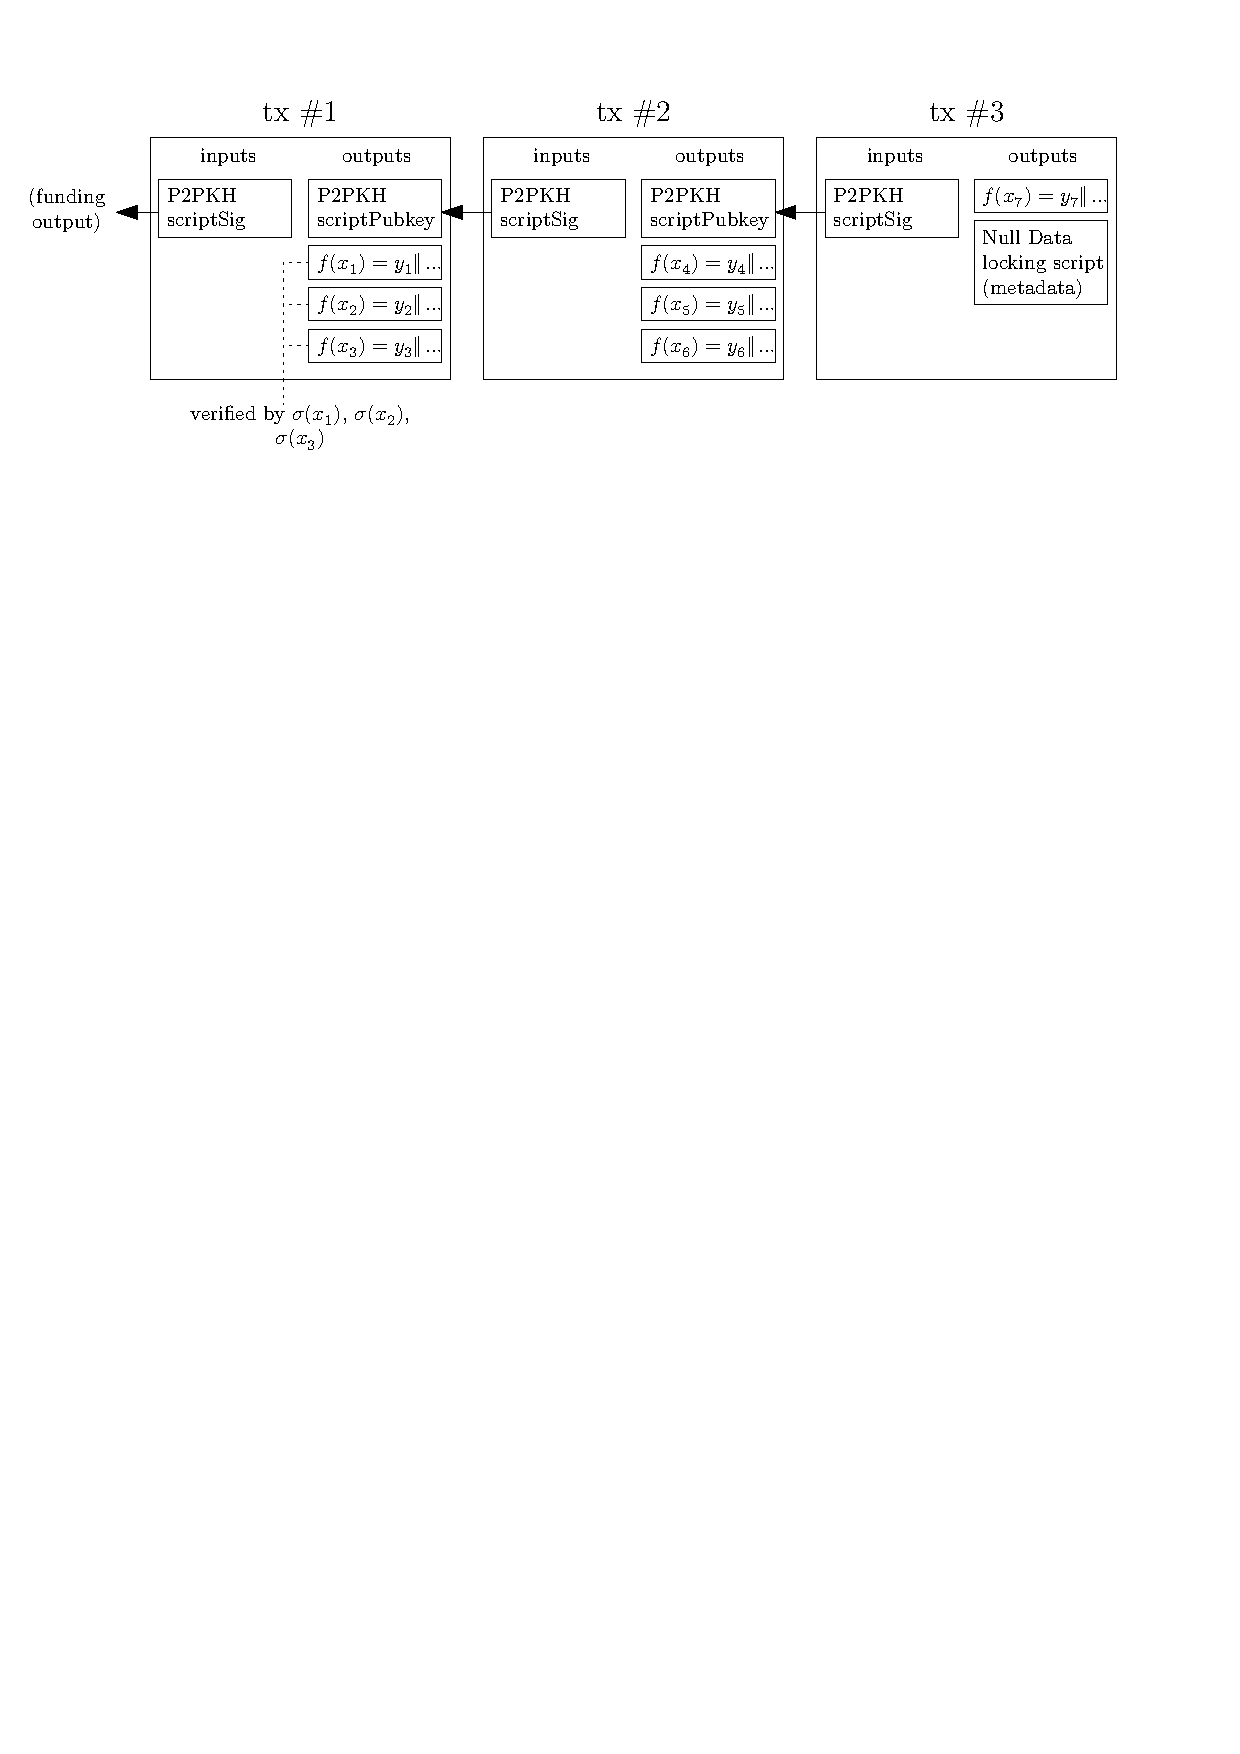
\includegraphics[width=16cm,keepaspectratio]{figure.pdf}
    \caption{}
\end{figure*}

\emph{Transaction construction.}
From assigned private keys, we can construct transactions containing the respective public keys $f(x_1), f(x_2), \dots$ in order, embedding the prefixes $y_1, y_2, \dots$.
That is, we construct a transaction with a single funding input, and add corresponding outputs containing the public keys as destination addresses, whereas every output must send a value of at least the non-dust amount of 546 sat.
If the size of the transaction exceeds a defined limit (or the network limit of $\SI{100}{\kilo\byte}$), we add an output refered by the next transaction as funding input, as depicted in figure \ref{fig:}.
A terminal OP\_RETURN-output allows embedding of metadata, facilitating reconstruction of the data.
Since we have chained the transactions using funding inputs, the transaction identifier of the last transaction can serve as locator for the data in the blockchain.
It is recommended to use P2PK(H) scripts as funding inputs, since the signatures in the scriptSig parts effectively prevents modifications to the transaction, for example an unwanted reordering of the transaction outputs.

\emph{Signature generation and submission.}
Again, having the private keys $x_1, x_2, \dots$, it is trivial to generate the proofs confirming ownership, e.g.\@ the signatures as defined by Seeg's countermeasure.
Submitting both the proofs and the previously generated transaction then successfully embeds the entire payload into the blockchain.
Note that this approach allows for the payload to be split up between multiple blocks in the blockchain.


\section{Increased cost of data inclusion}

After having demonstrated the possibility to circumvent the proposed countermeasure by brute force, this section attempts to evaluate the effectiveness of that countermeasure. 
Specifically, we assume a (not neccessarily adversarial) user, attempting to use the blockchain as data storage.
We will see that the user's chosen prefix length for the partial collissions directly determines the inclusion cost, hence we first model the inclusion cost mathematically. Then, by giving further estimations of essential parameters, we are able to predict by which factor the proposed countermeasure using proof-of-ownership signatures increases inclusion cost with respect to current, unprotected situation using fake addresses. 

\subsection{Modelling inclusion cost}

\begin{table*}[t]
    \centering
    \begin{tabular}{llr<{\,\si{\watt}}S[table-format=4.0,table-number-alignment=right]@{\,}rS[table-format=1.1e-2,table-number-alignment=right]r}
        \toprule
        \textbf{Method} & \textbf{Hardware} & \multicolumn{1}{r}{\textbf{est. wattage}} &\multicolumn{2}{r}{\textbf{est. freq.}} & \multicolumn{1}{r}{\textbf{$c$ in USD}} & \textbf{ref.}\cr
        %\midrule
        % TODO personal measures
        \midrule
        P2PKH & AMD RX 480  & 225 & 60 & \si{\mega\hertz} & 1.4e-13 &  Aug. 2016\cr %https://en.bitcoin.it/w/index.php?title=Vanitygen&type=revision&diff=61424&oldid=58554
              & GTX 1060  & 120 & 40 & \si{\mega\hertz} & 1.1e-13 &  Mar. 2018\cr
              & GTX 1080 TI  & 250 & 100 & \si{\mega\hertz} & 9.0e-14 &  Feb. 2019\cr
        \midrule
        P2SH & GTX 1080 TI & 250 & 2400 & \si{\mega\hertz} & 3.8e-15 & \cr % https://gist.github.com/epixoip/ace60d09981be09544fdd35005051505
        & RTX 2080 TI & 280 & 3800 & \si{\mega\hertz} & 2.7e-15 & \cr % https://gist.github.com/epixoip/ace60d09981be09544fdd35005051505
        & RTX Titan & 300 & 4300 & \si{\mega\hertz} & 2.5e-15 & \cr% https://gist.github.com/Chick3nman/5d261c5798cf4f3867fe7035ef6dd49f
        \bottomrule
    \end{tabular}
    \caption{User's reports of their brute-force frequencies on specific hardware. For the P2PKH method, frequency was directly taken from reported \emph{Vanitygen} speed. For the P2SH method, SHA256 hash frequency reported from \emph{Hashcat} was divided by factor 2, as explained in the respective section.
    We estimate cost parameter $c$ for the {P2PKH} by first researching estimated power consumption of the GPU under full load, and assuming energy cost of \num{.13} USD per \si{\kilo\watt\hour}.}
    \label{table:cost}
\end{table*}

Essentially, the choice of a suitable prefix length is a trade-off:
On the one hand, the number of required keypairs, and hence needed transaction fees, are inversely proportional to the chosen prefix length;
on the other hand, the probability for a partial collision decreases exponentially with respect to the prefix length, and in turn, computation cost increases exponentially.

To precicely model the cost of an inclusion of an arbitrary payload into the blockchain, restricted with the proposed countermeasure, let us denote 
\begin{itemize}
    \item prefix length with $n$,
    \item payload length with $N$,
    \item cost of a single hash operation with $c$,
    \item transaction fee for a single address with $f$.
\end{itemize}
Moreover, we denote $m=N/n$ as the number of required addresses, (or equivalently, the number of payload fragments) and $X$ as the random variable of required hash operations.
From this, total cost $C$ of an inclusion can be given with
\[ C =  c X + fm = c X + fN/n . \]

To precicely determine random variable $X$, we remind ourselves of the general iterative procedure of the brute-force algorithm:
In each iteration, the algorithm determines a keypair such that its prefix matches one of the payload fragments not yet assigned a keypair, and then assigns that fragment the keypair.
That is, in iteration $i$, the algorithm chooses private keys randomly, until generated public key paritially collides with one of the $m-i$ remaining unassigned payload fragments.
In the worst case, all fragments are pairwise different%
%\footnote{This is to be expected for sufficiently large prefix length $n$:}%
, hence one iteration can be viewed as repeated independent Bernoulli trials until success (i.e.\@ partial collision found), with success probability $(p-i)/2^n$.  
(This relies on the assumption that the generated public key is uniformly chosen from the resp.\@ codomain.)
Refering to required hashes in iteration $i$ with $X_i$, we thus observe that the random variable $X_i$ follows a geometric distribution with parameter $(p-i)/2^n$.
For the total number of required hash operations $X$, we reach (with $H_p$ the $m$-th harmonic number)
\[ X = \sum_{i=1}^{m} X_i, \quad E[X] = \sum_{i=1}^{m} E[X_i] = \sum_{i=1}^{m}\frac{2^n}{i} = 2^n\, H_m, \]
and conclude for the expected total cost $C$
\begin{equation}
    E[C] = 2^n\, H_m\,c + fm.\label{eq:totalcost}
\end{equation}

%Figure \ref{fig:xxx} plots the expected total cost with respect to chosen prefix length, using $N=\SI{1000}{\byte}$, and sensible values for $f$, $c$, assuming the {P2PK} method (cf. next section).
%We can clearly observe a minimum value, the inverse proportionality in bit ranges left of highlighted minimum value, and the exponential growth right of the minimum value.

\subsection{Estimation of parameters}

% TODO intros, Hardware?

%The software introduced in previous section was used to measure values for $c$, separately for each inclusion method ({P2PK, P2PKH, P2SH}).
%Additionally, we can give further estimates for cost $c$ indirectly for the inclusion method {P2PKH} and {P2SH}.

Before we can determine the cost increasse caused by the proposed countermeasure, we need to give sensible estimations for the cost parameters $c$ and $f$ involved in the previously stated cost model (\ref{eq:totalcost}).
While fees $f$ for publishing an address are directly determined by the miners' transaction fee rate, hashing cost depends on the efficiency of the hardware used for the brute-force process.
For this, we estimate the paramter indirectly using hash-rates reported by users of the tools \emph{Vanitygen} and \emph{Hashcat}.
%Since the P2PK method turns out to be the least effective, the omit an estimation of $c$ for this method.

\paragraph{Transaction fees}


\begin{table*}[t]
    \centering
    \begin{tabular}{lrrrS[table-format=2.2,table-alignment=right]rS[table-format=1.2e-1,table-alignment=right]}
        \toprule
        & \llap{script size} & max. payload & max. addresses & {tx bytes} & {non-dust amount} & {}\cr
        Type & in byte & length in byte & per tx &  {per address} & {per address in sat} & {$f$ in USD}\cr
        \midrule
        % TODO recalculate with input script length 72
        P2PK & 35 & 32 & 2267 & 44.10 & 546 & 7.78e-2\cr
        1-of-3 P2MS  & 105 & 32 & 2625 & 38.09& 182 & 4.44e-2\cr
        P2PKH & 25 & 20 & 2934 & 34.08 & 546 & 6.99e-2\cr
        P2SH & 23 & 20 & 3117 & 32.08& 546 & 6.83e-2\cr
        \bottomrule
    \end{tabular}
    % omit script size/payload size?
    \caption{Overview of the different trasaction types. 
        First column denotes the scripts size for a trasaction output, holding an address (resp. three addresses in the case of P2MS).
        Second column denotes the maximum payload length per address (in particular, the first byte of a 33-byte public key is a fixed prefix).
        Third column gives how many addresses can be gathered in a single transaction (not exceeding the size limit of \SI{100}{\kilo\byte}),
        fourth column the average bytes required per address in that particular transaction.
        Note that non-dust amount (546 sat) is counted by output, hence P2MS non-dust amount per address is one third.
    To compute value $f$, we multipy the transaction bytes required per address (column 5) with current miner's transaction fees (10 sat per byte), and add the smalles non-dust amount (column 6), converted at current exchange rate of \num{7.9e3} USD per bitcoin.}
\end{table*}

The fees required for publishing the address into the blockchain, i.e. parameter $f$, can easily estimated using average bytes required for a transaction output.
For this, we construct the largest possible transaction  using a single P2PK coinbase input to fund the outputs with non-dust burns, and adding outputs until reaching network's size limit of $\SI{100}{\kilo\byte}$.
Multiplying with miner's transaction fees, and adding smallest non-dust burn amount (dependent on method) yields the value for paramter $f$.
Table \ref{table:} gives this parameter in absolute values for all three methods, using transaction fees and Bitcoin exchange rate at point of publication.
That is, network's transaction fee of 10 sat per byte, and \num{7.9e3} USD per bitcoin.
Note that the P2MS strategy, arranging pubkeys in 1-of-3 multisig outputs, is currently the least expensive one in terms of fees required.
Even though multisig outputs cause more overhead in the constructed transaction, required non-dust amount is counted per output, hence, grouping three pubkeys into one transaction output saves on burnt bitcoins.

Since the P2PK method performs worst in this regard, we discard this method and focus on the related method P2MS, besides the fact that these two methods only differ in their transaction construction, yet are identical in their brute-force procedure.

\paragraph{P2PKH hash cost estimation}
For the {P2PKH} method, we can rely on user reports on their performance using the tool \emph{Vanitygen}, which allows users to create vanity addresses.
These Bitcoin addresses contain a human-readable prefix in their Base-58 representation.
Similiarly to the presented tool in previous section, \emph{Vanitygen} brute-forces private keys, until the hashed public key has the desired prefix;
this public key hash is preciely the one used to create {P2PKH} hashes.

Hence, due to the computational similarity, it seems reasonable to estimate possible computational cost for the {P2PKH} method from reported frequencies of \emph{Vanitygen} on selected hardware.
We assume that the computational effort of testing if a public key hash partially collides with one of the remaining unassigned payloads is negleglible.
In fact, the \emph{OpenCL} code used for the (usually faster performing) GPU code direcly builds on top of the one used in \emph{Vanitygen}.
Table \ref{table:cost} gives estimations for cost $c$ bases on selected user reports.

\paragraph{P2SH hash cost estimation}
In a similar matter, one can use the performances in computing {SHA256} digests as estimation for the cost of the {P2SH} method.
As was outlined in previous section, the brute-force procedure for the {P2SH} method constructs from nonce candidate $x$ a 57-byte long redeem script $S(x)$, and computes the {P2SH} address as the hash digest 
\begin{equation}
    x \mapsto \text{{RIPEMD160}}(\text{{SHA256}}(S(x))).\label{eq:p2sh-hash}
\end{equation}
% http://bench.cr.yp.to/results-hash.html#amd64-skylake
% https://en.wikipedia.org/wiki/Comparison_of_cryptographic_hash_functions
% KL15
The primitive hash functions {RIPEMD160} and {SHA256} are highly similar in architecture and performance; their respective Merkle–Damgård transforms also operate on the same block size of 512 bits.
Therefore, the effort required in above procedure (\ref{eq:p2sh-hash}) can be considered twice as large as one {SHA256} digest computation (in the sense of input length $\leq\!\SI{512}{\bit}$). 

% hashcat
Likewise to previous estimation using \emph{Vanitygen}, we can use hash frequencies published by users of the password cracking tool \emph{Hashcat}.
Dividing the reported SHA256 hash frequency by factor 2 thus yields an approximate frequency accomplishable for the P2SH brute-force procedure.
(We tacitly assume that the GPU can be programmed to perform RIPEMD160 calculations in similar speed.)
Again, refer to table \ref{table:cost} for estimations on cost $c$ bases on selected user reports.
Both the P2PKH and the P2SH method perform the same hash operations, only the former has to additionally perform a elliptic-curve addition.

Comparing the two methods, we can already observe that elliptic-curve arithmetics involved in the P2PK(H)/P2MS method heavily dominates the brute-force process.
We therefore omit a precise cost estimation of the P2PK/P2MS method, and can assume that savings made by omitting the RIPEMD160/SHA256 operations (in comparision to the P2PKH method) are neglegible.

\subsection{Comparison with state-of-the-art methods}

% TODO correct kilobyte mistake

\begin{figure*}[tb]
    \centering
    \pgfplotstableread[col sep=comma, ignore chars={"}]{graph1.csv}{\totalcostplot}
    \begin{tikzpicture}[
            mark size=1.5pt
        ]
        \begin{semilogyaxis}[
                height=8cm,
                width=13cm,
                grid=both,
                xmin=5,
                xmax=55,
                ymax=100,
                log ticks with fixed point,
                ymin=1,
                cycle list name=mylist,
                legend style={at={(0.5,0.95)},
		anchor=north,legend columns=2},
                xlabel={Prefix length $n$ in bits},
                ylabel={Expected cost per kilobyte in USD}
            ]

            \addplot+[mark=x] table [x={n}, y={p2pkh}] {\totalcostplot};
            \addlegendentry{P2PKH}
            \addplot+[mark=o] table [x={n}, y={p2ms}] {\totalcostplot};
            \addlegendentry{P2MS}
            \addplot+[mark=square] table [x={n}, y={p2sh}] {\totalcostplot};
            \addlegendentry{P2SH}
            \addplot+[dashed,mark=none] table [x={n}, y={p2fms}] {\totalcostplot};
            \addlegendentry{fake multisig}
        \end{semilogyaxis}
    \end{tikzpicture}
    \caption{Log-linear plot of expected total cost $\mathrm{E}[C]$ (see equation \ref{eq:totalcost}) with $N=\SI{10}{\kilo\byte}$ for inclusion methods P2PKH ($c=\num{1.0e-13}$ USD, $f=\num{6.99e-2}$ USD), P2MS ($c=\num{1.0e-13}$ USD, $f=\num{4.44e-2}$ USD), P2SH ($c=\num{3.0e-15}$ USD, $f=\num{6.83e-2}$ USD). For comparison, dotted line indicates constant efficiency achievable using fake addresses in multisig outputs.}
\end{figure*}

This section compares the impact of the proposed inclusion method with the current situation, having no countermeasures.
To begin with, we choose following rough but sensible estimates for computation cost parameter $c$ for methods P2MS, P2PKH, P2SH, based on our observations from previous section.
We estimate $c_\text{ms}=c_\text{pkh}=\num{1.0e-13}$ USD, $c_\text{sh} = \num{3.0e-15}$ USD.
Also stated in previous section, fee parameter $f$ directly follows from Bitcoin exchange rate and mining fees, and is displayed in table \ref{table:}.

As was given in the introduction, the best present method of including arbitrary data uses fake public keys (in their extended 65 byte representation) arranged in 1-of-3 multisig outputs, not being inhibited by any countermeasure requiring proof signatures.
Relative cost of inclusion using this state-of-the-art method can easily be estimated using same formula (\ref{eq:totalcost}), assigning $c=0$, maximum prefix size $n=\SI{65}{\bit}$, and computing $f$ identically to previous procedure, considering \SI{70.16}{\byte} per 65-byte-address/-pubkey.
This gives us a constant cost efficiency of \num{1.07e-3} USD per byte as benchmark.

Figure \ref{fig:plot} plots the expected cost per byte payload, using $N=\SI{10}{\kilo\byte}$ and previously stated parameters, for each method.
As comparison, the constant relative cost of the state-of-the-art method is highlighted by the dashed horizontal line. 

We confirm that determiniong the most cost-effetive prefix length corresponds to finding the local minimum of the cost function.
Futhermore, the plot supports the trade-off nature of the problem: left of the maximum point, cost increases proportional due to more addresses required; cost right of the maximum point is dominated by the exponentially increasing brute force computation cost.

By routine exhaustion, we give minimum cost per kilobyte payload in table \ref{table:},
and obtain following result: 
defending the Bitcoin network against unwanted data inclusion using proof-of-ownership signatures could allow for an 8-fold increase of inclusion cost, at current situation.

Nevertheless, it needs to be highlighted that optimal cost efficiency can only be obtained using significant computational power.
For example, using the fastest GPU for the P2SH inclusion method from table \ref{table:}, including the \SI{10}{\kilo\byte} already requires 72 hours of computation.
In fact, real-time inclusion using non-specialized hardware seems out of reach for prefix lenghts as low as 28 bits, requiring more than a minute of computation time on a typical personal computer for payload length of $N=\SI{100}{\byte}$ (assuming hash frequency of \SI{10}{\mega\hertz}).

\begin{table}
    \centering
    \begin{tabular}{lrS[table-format=0.4,table-alignment=right]S[table-format=2.2,table-alignment=right]}
        \toprule
        & {\textbf{\llap{opt. prefix}}} & {\textbf{exp. cost in}} & \textbf{{rel. increase}}\cr
        & {\textbf{length}} & {\textbf{USD per kB}} & {\textbf{w.r.t.\@ P2FMS}}\cr
        \midrule
        P2MS  & 42 & 8.82 & 8.21\cr
        P2SH & 47 & 12.0 & 11.2\cr
        P2PKH & 42 & 13.7 & 12.7\cr
        \bottomrule
    \end{tabular}
    \caption{Minimum point $n$ and minimum value $\mathrm{E[C]}$ from plot in figure \ref{fig:}. Rightmost column gives the relative increase with respect to the constant efficiency achievable using fake addresses in multisig outputs.}
\end{table}



\subsection{Variations in parameters}

We established a model estimating cost of inclusion from parameters $N$, $f$ and $c$, corresponding to payload size resp.\@ the economic situation of the Bitcoin network (transaction fees, bitcoin exchange rate) resp.\@ computational cost of the hashing procedure.
It is therefore logical to investigate the impact on changes on this parameter, especially since a continuiation of the exponentially growing trend of computation efficiency is expected, and many believing a significant increase in bitcoin's exchange rate.
To keep the analysis reasonable, we restrict the parameter space to $10^{-20} \leq c \leq 10^{-12}$ for computation cost, and for the bitcoin price $p$ to range $\SI{1000}\,\text{USD}/\text{BTC} \leq p \leq 10^6\,\text{USD}/\text{BTC}$.
Due to the transcendental nature of the cost function $\mathrm{E}[C]$ with respect to prefix length $n$, it seems out of reach to formulate a closed-form solution to finding optimal prefix length and respective total cost, given parameters $N$, $f$, $c$.
Hence, numerical methods are applied to determine minimal cost, given numerical values of the parameters.

Before discussing the impact of $p$ and $c$, we can observe that relative savings from larger payload size $N$ are effectively negleglible, that is, total cost is near-linear with respect to payload size;
this trend is independent of all other parameters.
Therefore, we continue our analysis by looking at the cost of an inclusion \emph{relative} to payload size.

In order to derive parameter $f$ from bitcoin exchange rate $p$, we fix the P2MS method and network transaction fees of 10 sat per byte.
From this, as was alreay performed in section \ref{}, we define $f = p \cdot (182\,\text{sat} + \SI{38.09}{\byte}\cdot 10\,\text{sat}\,\si{\per\byte})$, that is, again, non-dust amount per address plus bytes occupied in the transaction multiplied with network fees.
Combining with given parameter $c$, let $C_\text{p2ms}(p,c)$ be the optimal relative inclusion cost in USD per byte, determined by numerically finding optimal prefix length $n$.

In order to state the effect of bitcoin price and computation cost quantitatively, we proceed with numerically computing $C_\text{p2ms}(p,c)$ for $c$ and $p$ in the peviously fixed respective ranges; price $p$ in $10^{0.5}$-fold increments, $c$ in $10^{0.2}$-fold increments, yielding 272 data points.

We continue by presenting a bivariate log-log regression model to explaining the dependent data points from the independent varaibles, that is,
\[ \log_{10} \frac{C_\text{p2ms}(p, c)}{\text{USD}\,\si{\per\byte}} = \alpha + \beta \log_{10} \frac{p}{\text{USD}} + \gamma \log_{10} \frac{c}{\text{USD}} + \epsilon_i, \]
with unknown parameters $\alpha$, $\beta$, $\gamma$, and error terms $\epsilon_i$.
Usual least-squares-error method provides $\alpha \approx \num{5.342}$, $\beta \approx\num{0.9731}$, $\gamma \approx\num{.0267}$.

It is explicitly to be remarked that this model does not precicely explain the data; this becomes clear when considering the visible patterns in the residual graph of this regression.
Nevertheless, the model appears to be sufficiently precise to estimate the effect of the varaibles $p$, $c$ on relative inclusion cost: in fact, mean square error $\sum \epsilon_i^2/(n-2) < \num{e-4}$, and maximum residual is $\max |\epsilon_i| < 0.022$. Consequently, the model predicts inclusion cost with a relative error of at most \SI{5.2}{\percent}.
See also figure \ref{}, which plots observed data points against the fit in a log-log plot.

Having established that model, we can derive from parameters $\beta$ and $\gamma$ following observations.
First, as we expected, relative inclusion cost $C_\mathrm{p2sh}(p,c)$ is almost linear.
Since sublinear, we expect that $C_\mathrm{p2sh}(p,c)$ continues to converge towards inclusion cost reachable using fake keys, which grows linear w.r.t.\@ price $p$.
Nevertheless, this trend appears to be minor; a 100-fold bitcoin price increase lowers relative inclusion cost by no more than \SI{12}{\percent}.

Second, computation cost $c$ has – independent of bitcoin price $p$ – only slim effects on inclusion cost: lowering computation cost by factor $10^6$, for example, would lead to a relative inclusion cost of $\SI{69}{\percent}$ of original computation cost. (Moore's law estimates the cost decrease of factor $10^6$ in a timespan of 40 years.)

We conclude: even though effectiveness of the proposed countermeasure decreases both with increasing bitcoin price and decreasing computational cost, effectiveness remains stable even for extreme values.
For our established bounds of parameters, this means $C_\mathrm{p2sh}(p,c) / C_\mathrm{fake}(p) \geq \num{7.3}$.

% TODO it is clear that cost using fake keys scales linear
%Similarly, relative cost of data inclusion using fake keys $C_\text{fake}$ can be generalized similarly from section \ref{}, we reach
%\begin{align*}C_\text{fake}(p) &= p\cdot\left(182\,\text{sat} + \SI{70.16}{\byte}\cdot 10\,\text{sat}\,\si{\per\byte}\right)\cdot \SI{65}{\per\bit}\\
    %&\approx p\cdot \num{460}\,\text{sat}\,\si{\per\kilo\byte}.
%\end{align*}




% Trends: better hashing performance -> lower c, possible increase in fees and bitcoin price -> higher f
% savings with larger N are nearly negleglible



\section{Cost of malicious attack}

In this section, we address the problem of data inclusion from the perspective of a malicious adversary.
As was outlined in the introduction, deliberate inclusion of problematic data into the Blockchain, such as copyright-protected, illegal, or politically sensitive content, could render the possession of the Blockchain illegal in most jurisdictions.
Hence, due to persistency of the blockchain, this malicious inclusion harms every participant in Bitcoin's network, and might make participation even legally impossible.

Since Bitcoin's concensus mechanism is the basis for its security, we assume a consensus attack (i.e. \textquote*{51\%-attack} – controling more than honest miner's hashrate) as an upper bound for a disruptive attack against Bitcoin's network.
Therefore, we evaluate the cost of such an attack including malicious content \emph{in terms of computational power}.
It seems adequate to measure the required computational power \emph{relative to the concensus attack}.
Focusing on computation resources, we ignore any monetary cost associated with publishing transactions to the blockchain, e.g. miners' transaction fees and burnt non-dust outputs.

% https://www.vice.com/en_us/article/d73b8k/the-mystery-behind-the-biggest-bitcoin-transaction-ever-made
% https://arstechnica.com/tech-policy/2017/12/bitcoin-fees-rising-high/
Nevertheless, we restrict the attack to publishing only one transaction of size \SI{10}{\kilo\byte} per block, occupying \SI{1}{\percent} of the block's capacity.
Allowing the attacker to publish larger transactions might cause signifcant increases in transaction fees, and secondly, would effectively transform this type of attack into a flood attack, which is not subject of discussion.
Although this could potentially be bypassed by solo-mining blocks with respective payload-carrying transactions, provided sufficient computational power, this would similarly transform this approach to a concensus attack.

\paragraph{Comparing computational effort}
As we have already seen, data inclusion using {P2SH} addresses via brute-forcing many redeem scripts is the computationally least expensive method.
To compare the computational cost to Bitcoin's mining process, we argue that the expense of hashing a single {P2SH} transaction is comparable to hashing a single block header during the Proof-of-Work mining process.
% TODO
%Only as a theoretical consideration, we can build an additional estimation on the basis of Bitcoin mining hardware.
%The emergence of mining hardware developed using application-specific integrated circuits (ASIC) proved that SHA-256 hashes can be computed with an efficiency magnitudes better than traditional GPU-based methods.
%Nevertheless, reliable numbers for the efficiency of such ASIC units seem to only appear in the context of Bitcoin mining, therefore, we focus on such mining hardware.
%It has to be emphasized that the advertized strong computation power of such ASIC units cannot directly be utilized for the task of performing the P2SH computation (\ref{eq:p2sh-hash}), and the determined numbers only serve as an indirect estimation of the theoretical efficiency permitted by application-specific integrated circuits.
%
In comparison to the P2SH hash procedure (\ref{eq:p2sh-hash}), Proof-of-Work mining constructs from nonce candidate $x$ the 80-byte long block header $H(x)$, and performs a double SHA-256 hashing, i.e. 
\begin{equation}
    x \mapsto \text{{SHA256}}(\text{{SHA256}}(H(x))),\label{eq:pow-hash}
\end{equation}
to test against network target.
We alread argued in section \ref{sec:parameter-estimation} that P2SH hashing (\ref{eq:p2sh-hash}) requires computational work comparable to two SHA256 calculations; from above construction (\ref{eq:pow-hash}) follows the stated claim that computing a P2SH hash is approximately as hard as computing a Proof-of-Work hash.

This conclusion is not immediate due to following apparent caveat: block headers $H(x)$ are substantially longer than redeem scripts $S(x)$.
As the former input is split into two 512-bit blocks for hashing, computation requires two invocations of the respective {SHA256} compression function in the Merkle–Damgård transform.
However, the first 512 bits of input $H(x)$ remain constant with respect to chosen nonce $x$, and in general, during mining, the \textquote*{mid-state} after applying the first compression is precomputed and stored.
Hence, computations of $\text{{SHA256}}(S(x))$ and $\text{{SHA256}}(H(x))$ both require only a single invocation of the compression function.
% https://link.springer.com/chapter/10.1007/978-3-662-44893-9_12

\paragraph{Payload data rate}
Let us denote $r$ (bit per second) as the targeted rate of payload to be included into the blockchain.
As we have agreed to a transaction's size limit of \SI{10}{\kilo\byte}, at most $p=308$ addresses can be published per block, i.e., for given prefix lenght $n$, $np$ bit per block, or per 10 minutes. 

From this, required prefix length $n=\SI{10}{\minute}\cdot r/p$ directly follows when attaining data rate $r$.
This, in turn, requires the brute-force process to produce $p$ suitable addresses in no longer than 10 minutes, in order to submit the corresponding transaction in the following block.

\begin{table}[]
    \centering
    \begin{tabular}{rS[table-format=1.2,table-number-alignment=right]rS[table-format=2.1,table-number-alignment=right]r}
        \toprule
        {\textbf{hash rate}} & \multicolumn{4}{c}{\textbf{payload data rate in \si{\byte\per\second}}} \cr
        \midrule
                    & \multicolumn{1}{r}{tx \SI{10}{\kilo\byte}} & ($n$) & \multicolumn{1}{r}{tx \SI{100}{\kilo\byte}} & ($n$) \cr
                    & {$p=308$} & & {$p=3117$} & \cr
        \midrule
        \SI{5}{\giga\hertz}& 2.49 & (38.8) & 24.9 & (38.3) \\
        \SI{20}{\tera\hertz}& 3.26 & (50.8) & 32.7 & (50.3) \\
        \SI{1}{\percent} & 4.25 & (66.2) & 42.7 & (65.8) \\
        \SI{10}{\percent} & 4.46 & (69.5) & 44.9 & (69.1) \\
        \SI{100}{\percent} & 4.68 & (72.9) & 47.1 & (72.4) \\
        \midrule
        (unrestr.) & 10.2 & (160) & 104 & (160) \\
        \bottomrule
    \end{tabular}
    \caption{Attainable rate of payload data included into the blockchain while circumventing proof-of-ownership countermeasure using proposed brute-force method on P2SH addresses, constrained by hash rate given in the left column. Percentages in the left column represent fractions of current total miners' hash rate (\SI{90}{\exa\hertz}). Second row shows the assumed maximum allowed transaction size for including addresses, per block.
    Last row calculates the payload data rate in absence of any countermeasure, i.e. using all 160 bits of the P2SH address field.}
\end{table}

Alluding to expected cost $\mathrm{E}[C]$, we can estimate expected computation time $\mathrm{E}[T]$ given prefix lenght $n$ and attacker's available hash rate $\nu$ with 
\[ \mathrm{E}[T] = 2^n\, H_p / \nu \leq \SI{10}{\minute}, \]
solving for $\nu$ yields $\nu \geq 2^n\cdot H_p / (\SI{10}{\minute})$.
In fact, this calculation demonstrates that a one-one mapping between hash rate and data rate exists: given $\nu$, we can calculate maximum prefix length $n$ and hence maximum attainable data rate.
Table \ref{} gives some numerical values, % additionally computed vor a transactions' size limit of \SI{100}{\kilo\byte} (i.e. the network's transaction size limit, and \SI{10}{\percent} of the block size limit).
Note that fractional prefix lengths $n$ were explicitly permitted, representing the \textquote*{average} prefix length, such that the computation time limit of 10 minutes is completely exploited.

We collect the following observation:
for brute-force hash rates currently attainable in practice using a GPU ($\nu = \SI{5}{\giga\hertz}$, first row of table \ref{}, see also table \ref{}), potential payload data rate drops to about \SI{24}{\percent}, relative to the data rate reachable by current methods which are not hindered by countermeasures (see last row).
Similarly, hash rate of currently available ASIC mining equipment ($\nu = \SI{20}{\tera\hertz}$, second row) could, only in theory, reach performances of \SI{32}{\percent}.
Do note however that current proof-of-work mining equipment fundamentally builds upon highly specialized integraded circuits – 
their efficiency cannot be used for the proposed brute-force procedure, and only serves as an indirect estimation of the theoretical efficiency permitted by application-specific integrated circuits.

% We conclude that, while proof-of-ownership countermeasures do cause a drop in attainable rate of (potentially harmful) data embedded into the blockchain, figures remain in a 

\section{Discussion and Conclusion}

% https://link.springer.com/article/10.1007/s11227-018-2317-6

\end{document}
